\documentclass{article}

\usepackage{pandekten}
\usepackage{dashrule}

\makeatletter
\newcommand*{\shifttext}[1]{%
  \settowidth{\@tempdima}{#1}%
  \hspace{-\@tempdima}#1%
}
\newcommand{\plabel}[1]{%
\shifttext{\textbf{#1}\quad}%
}
\newcommand{\prule}{%
\begin{center}%
\hdashrule[0.5ex]{.99\linewidth}{1pt}{1pt 2.5pt}%
\end{center}%
}

\makeatother

\newcommand{\minusbaseline}{\abovedisplayskip=0pt\abovedisplayshortskip=0pt~\vspace*{-\baselineskip}}%

\setlength{\parindent}{0pt}

\title{Final}
\author{}

\begin{document}

\maketitle

\plabel{A1 (a)}%
Denote by $d' = n d$, and assume that $r_d<0$ and no half-wave loss at the $r=1$ surface (since $r=1$), then
\[ \Gamma_{GT} = r_d + T e^{2ikd'} - r_d T e^{4ikd'} + r_d^2 T e^{6ikd'} - \cdots = \frac{r_d+e^{2ikd'}}{1+r_d^{2ikd'}}. \]

\plabel{(b)}%
Since $\abs{\Gamma_{GT}}^2 = 1$, this is a total reflection and is therefore one-port.
It's clear that $\abs{S_{11}}^2 = 1$.

\plabel{(c)}%
\begingroup\minusbaseline
\begin{align*}
    \Re S_{11} &= \frac{2 r_d + \left(r_d^2+1\right) \cos (2 k d')}{1+r_d^2 + 2 r_d \cos (2 k d')} = \frac{2 r_d + \left(r_d^2+1\right) \cos (\delta)}{1+r_d^2 + 2 r_d \cos (\delta)}, \\
    \Im S_{11} &= -\frac{\left(r_d^2-1\right) \sin (2 k d')}{1+r_d^2+2 r_d \cos (2 k d')} = -\frac{\left(r_d^2-1\right) \sin (\delta)}{1+r_d^2+2 r_d \cos (\delta)}.
\end{align*}
\endgroup

\plabel{(d)}%
From
\[ \Phi = 2\arctan(\sigma\tan(\frac{\omega}{c} n d)) \]
we find
\[ \dv{\Phi}{\omega} = \frac{2 n d \sigma}{c} \cdot \frac{2}{1+\sigma^2 - (\sigma^2 - 1)\cos(\delta)}. \]
\begin{center}
    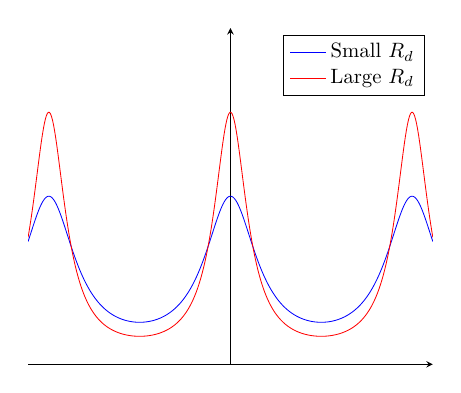
\begin{tikzpicture}[scale=0.75]
        \begin{axis}[
            axis x line=center,
            axis y line=center, 
          domain=-7:7,
          ticks=none,
          xmin=-7, xmax=7,
          ymin=-0, ymax=2,
          samples=400,
        ]
          \addplot+[mark=none]
            {2/(5-3*cos(deg(x)))};
        \addplot+[mark=none]
            {3/(10-8*cos(deg(x)))};
        \legend{Small $R_d$, Large $R_d$}
        \end{axis}
    \end{tikzpicture}
\end{center}
Dispersion is maximized at $\delta = 2 \pi \cdot (\text{integers})$.

\plabel{(e)}%
The peaks of $\displaystyle\dv{\Phi}{\omega}$ become higher.
Interference becomes stronger inside the etalon.

\plabel{(f)}%
\begingroup\minusbaseline
\begin{align*}
    \dv[2]{\Phi}{\omega} &= -\frac{4(nd)^2\sigma(\sigma^2-1)}{c^2} \frac{\tan(\delta/2)}{\cos^2(\delta/2)(1+\sigma^2 \tan^2(\delta/2))^2}.
\end{align*}
\endgroup
GDD vanishes when group delay is at a maximum.
\[ \dd{\dv{\Phi}{\omega}} \sim \dd{\delta} \]
with a negative coefficient.

\prule

\plabel{B1 (a)}%
\begingroup\minusbaseline
\begin{align*}
    H &= \begin{pmatrix*}
        \hbar\omega_1 & 0 & V_{13} \\
        0 & \hbar\omega_2 & V_{23} \\
        V^*_{13} & V^*_{23} & \hbar\omega_3
    \end{pmatrix*}, \\
    V_{12} &= -q_e(E_a \cos (\omega_{13}t) + E_b \cos(\omega_{23}t))\bra{1} x \ket{3}, \\
    V_{23} &= -q_e(E_a \cos (\omega_{13}t) + E_b \cos(\omega_{23}t))\bra{2} x \ket{3}.
\end{align*}
\endgroup
With the slow variables $c_i = \tilde{c}_i e^{-i\omega_i t}$ we find
\begin{align*}
    \dot{\tilde{c}}_1 &= \frac{i}{\hbar} {q_e \bra{1} x \ket{3}} \tilde{c}_3\qty(E_a \frac{1+e^{2i\omega_{13}t}}{2} + E_b \frac{e^{i(\omega_{13}+\omega_{23})t} + e^{i\omega_{12}t}}{2}), \\
    \dot{\tilde{c}}_2 &= \frac{i}{\hbar}{q_e \bra{2} x \ket{3}} \tilde{c}_3 \qty(E_a \frac{e^{i(\omega_{13}+\omega_{23})t} + e^{-i\omega_{12}t}}{2} + E_b \frac{1+e^{2i\omega_{23}t}}{2}), \\
    \dot{\tilde{c}}_3 &= \frac{i}{\hbar} {q_e \bra{3} x \ket{1}} \tilde{c}_1 \qty(E_a \frac{1+e^{-2i\omega_{13}t}}{2} + E_b \frac{e^{-i(\omega_{13}+\omega_{23})t} + e^{-i\omega_{12}t}}{2}) \\
    &{\phantom{{}={}}} + \frac{i}{\hbar}{q_e \bra{3} x \ket{2}} \tilde{c}_2 \qty(E_a \frac{e^{-i(\omega_{13}+\omega_{23})t} + e^{i\omega_{12}t}}{2} + E_b \frac{1+e^{-2i\omega_{23}t}}{2}).
\end{align*}

\plabel{(b)}%
Under RWA
\begin{align*}
    \dot{\tilde{c}}_1 &= \frac{i}{2 \hbar} q_e \bra{1} x \ket{3} (E_a + E_b) \tilde{c}_3, \\
    \dot{\tilde{c}}_2 &= \frac{i}{2 \hbar} q_e \bra{2} x \ket{3} (E_a + E_b) \tilde{c}_3, \\
    \dot{\tilde{c}}_3 &= \frac{i}{2 \hbar} q_e \bra{3} x \ket{1} \tilde{c}_1 (E_a+E_b) + \frac{i}{2 \hbar} q_e \bra{3} x \ket{2} (E_a + E_b) \tilde{c}_2.
\end{align*}
\begin{itemize}
    \item $\lambda_1 = 0$ has eigenvector
    \[ \psi_1 = \frac{1}{\sqrt{\abs{\bra{1} x \ket{3}}^2 + \abs{\bra{2} x \ket{3}}^2}} \begin{pmatrix}
        \bra{3} x \ket{2} \\
        -\bra{3} x \ket{1} \\
        0
    \end{pmatrix}. \]
    \item $\displaystyle \lambda_2 = i\frac{q_e}{2\hbar} (E_a + E_b) \sqrt{\abs{\bra{1} x \ket{3}}^2 + \abs{\bra{2} x \ket{3}}^2}$ has eigenvector
    \[ \psi_2 = \frac{1}{\sqrt{2(\abs{\bra{1} x \ket{3}}^2 + \abs{\bra{2} x \ket{3}}^2)}} \begin{pmatrix}
        \bra{1} x \ket{3} \\ \bra{2} x \ket{3} \\ \sqrt{\abs{\bra{1} x \ket{3}}^2 + \abs{\bra{2} x \ket{3}}^2}
    \end{pmatrix}. \]
    \item $\displaystyle \lambda_2 = -i\frac{q_e}{2\hbar} (E_a + E_b) \sqrt{\abs{\bra{1} x \ket{3}}^2 + \abs{\bra{2} x \ket{3}}^2}$ has eigenvector
    \[ \psi_3 = \frac{1}{\sqrt{2(\abs{\bra{1} x \ket{3}}^2 + \abs{\bra{2} x \ket{3}}^2)}} \begin{pmatrix}
        \bra{1} x \ket{3} \\ \bra{2} x \ket{3} \\ -\sqrt{\abs{\bra{1} x \ket{3}}^2 + \abs{\bra{2} x \ket{3}}^2}
    \end{pmatrix}. \]
\end{itemize}
Denote the solution by
\[ \alpha_1 e^{\lambda_1 t} \psi_1 + \alpha_2 e^{\lambda_2 t} \psi_2 + \alpha_3 e^{\lambda_3 t} \psi_3 \]
we find
\begin{align*}
    \alpha_1 &= \frac{\bra{2} x \ket{3} \cos\theta - \bra{1} x \ket{3} \sin\theta}{{\abs{\bra{1} x \ket{3}}^2 + \abs{\bra{2} x \ket{3}}^2}}, \\
    \alpha_2 = \alpha_3 &= \frac{\bra{3} x \ket{1} \cos\theta + \bra{3} x \ket{2} \sin\theta}{\sqrt{2} \qty({\abs{\bra{1} x \ket{3}}^2 + \abs{\bra{2} x \ket{3}}^2})}.
\end{align*}

\plabel{(c)}%
We need
\[ \bra{3} x \ket{1} \cos\theta + \bra{3} x \ket{2} \sin\theta = 0, \]
i.e.
\[ \tan\theta = -\frac{\bra{3}x\ket{1}}{\bra{3}x\ket{2}}. \]

\plabel{(d)}%
With detuning, $\theta$ becomes smaller.

\prule

\plabel{B2 (a)}%
\begingroup\minusbaseline
\begin{align*}
\dot{D}(x,t) &= -\gamma_{\parallel} (D(x,t) - D_0) + \frac{2i}{\hbar} E(x,t) [P^{-}(x,t) - P^{+}(x,t)]\\
&=-\gamma_{\parallel} (D(x,t) - D_0) + \frac{2i}{\hbar} \sum_{m,m'} [E_m P^*_{m'} e^{i(\Omega_{m'}-\Omega_m) t} - \mathrm{h.c.}].
\end{align*}
\endgroup
In the stationary case we discard all terms with $\Omega_{m'}\neq \Omega_m$.

\plabel{(b)}%
\begingroup\minusbaseline
\begin{align*}
0 &= (-i\omega_{12} - \gamma_{\perp} )P(x,t) - i\frac{\mathcal{P}_{12}^2}{\hbar}E(x,t)D(x,t), \\
-\sum_{m=1}^N i\Omega_m P_m(x) e^{-i\Omega_m t} &=(-i \omega_{12} - \gamma_{\perp})\sum_{m=1}^N P_m(x)e^{-i\Omega_m t} \\
&{\phantom{{}={}}} -i\frac{\mathcal{P}_{12}^2}{\hbar} \sum_{m=1}^{N} E_m(x) e^{-i\Omega_m t}D_{ss}.
\end{align*}
\endgroup
With the stationary condition we match the components and find
\begin{align*}
P_m(x) &= \frac{-\frac{i\mathcal{P}_{12}^2}{\hbar}E_m(x)D_{ss}(x)}{-i(\Omega_m - \omega_{12}) + \gamma_{\perp} }.
\end{align*}

\plabel{(c)}%
Under stationary condition we obtain
\begin{gather*}
-\gamma_{\parallel} (D_{ss} - D_0) + \frac{2i}{\hbar} \sum_{m=1}^N [E_m P^*_{m} - \mathrm{h.c.}] = 0, \\
-\gamma_{\parallel} (D_{ss} - D_0) - \frac{4\mathcal{P}_{12}^2 \gamma_{\perp}}{\hbar^2}\qty[\sum_{m=1}^N \frac{\abs{E_m}^2}{(\Omega_{m}-\omega_{12})^2 + \gamma_{\perp}^2}]D_{ss} = 0, \\
D_{ss} = \frac{D_0}{1 + \frac{4\mathcal{P}_{12}^2 \gamma_{\perp}}{\hbar^2 \gamma_{\parallel}}\sum_{m=1}^N \frac{\abs{E_m}^2}{(\Omega_{m}-\omega_{12})^2 + \gamma_{\perp}^2}}.
\end{gather*}

\plabel{(d)}%
\begingroup\minusbaseline
\begin{gather*}
    \qty[\grad^2 + \frac{n^2}{c^2}\Omega_m^2] E_m(x) = -\frac{n^2}{c^2 \epsilon_0}\Omega_m^2 P_m(x) \\
    \qty[\grad^2 + \frac{n^2}{c^2}\qty(1+ P_m(x)/\epsilon_0E_m) \Omega_m^2]E_m(x) = 0.\\
    n_{\text{eff}}^2 = n^2\qty(1- \frac{\frac{i\mathcal{P}_{12}^2}{\hbar}}{-i(\Omega_m - \omega_{12}) +\gamma_{\perp} }\frac{D_0}{1 + \frac{4\mathcal{P}_{12}^2 \gamma_{\perp}}{\hbar^2 \gamma_{\parallel}}\sum_{m=1}^N \frac{\abs{E_m}^2}{(\Omega_{m}-\omega_{12})^2 + \gamma_{\perp}^2}}).
\end{gather*}
\endgroup

\plabel{(e)}%
$n_{\text{eff}}^2$ increases in the real part of but decreases in the imaginary part.

\plabel{(f)}%
\begingroup\minusbaseline
\begin{center}
    \begin{tikzpicture}[scale=0.75]
        \begin{axis}[
            axis x line=center,
            axis y line=center,
            %axes=none,
          domain=0:pi,
          ticks=none,
          xmin=0, xmax=pi,
          ymin=-0, ymax=1.5,
          samples=400,
        ]
          \addplot+[mark=none]
            {1/(1+sin(deg(x))^2 + sin(deg(2*x))^2/2)};
        \end{axis}
    \end{tikzpicture}
\end{center}
\endgroup
It's spatial hole burning.
 
% \bibliographystyle{plain}
% \bibliography{main}

\end{document}

